\chapter{Экспериментальные методы}\label{ch:ch2}

\section{Молекулярно-пучковая эпитаксия (МПЭ)}\label{sec:ch2/sec1}

Изучаемые в данной работе наноструктуры синтезированы методом МПЭ, в основе
которого лежит взаимодействие пучков атомов или молекул с кристаллической
подложкой в условиях сверхвысокого вакуума \((\sim 10^{-10}\)~\si{\torr}). При
таких давлениях длина свободного пробега молекул намного превышает
геометрические размеры реактора. Данная технология позволяет снизить
концентрацию инородных включений в синтезированных гетероструктурах,
контролировать толщину слоев и профиль легирования на уровне атомных размеров.

Структуры синтезировались на установке МПЭ Veeco GEN III
(см.~рис.~\cref{fig:Image_10}). Установка состоит из трёх высоковакуумных
камер: загрузочной (остаточное давление \(\sim 10^{-8}\)~\si{\torr}),
промежуточной (\(\sim 10^{-10}\)~\si{\torr}) и ростовой (\(\sim
10^{-10}\)~\si{\torr}). Откачка осуществляется турбиной, крионасосом,
магниторазрядным и титановым сублимационным насосами.

\begin{figure}[ht] \centerfloat{
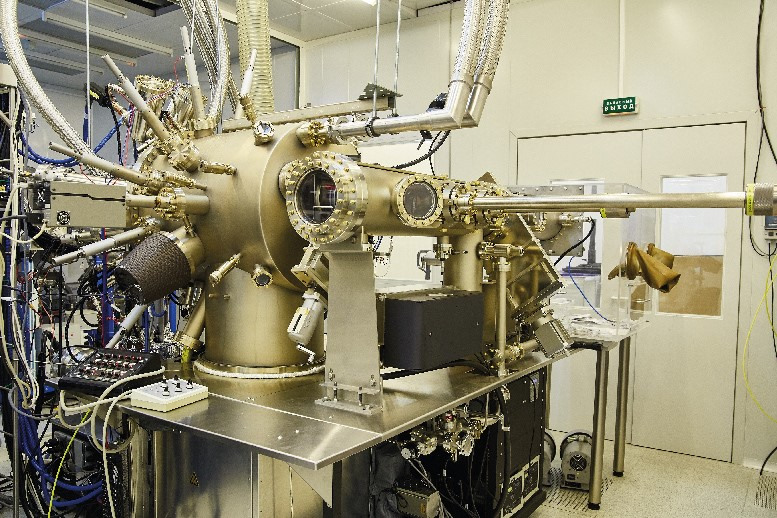
\includegraphics[width=0.6\linewidth]{Image_10} } \caption{Установка МПЭ Veeco
GEN III}\label{fig:Image_10} \end{figure}

Для поддержания высокого вакуума и предотвращения взаимного нагрева источников
ростовая камера в дополнение к насосам оснащена криопанелью~--- ёмкостью с
протекающим в ней жидким азотом. Криопанель эффективно адсорбирует частицы
остаточного газа в ростовой камере из-за низкой температуры своих стенок.

Давление в камерах контролируется ионизационными вакуумными датчиками
Байярда\,--\,Альперта, калиброванными по N\textsubscript{2}. Принцип их
действия: электроны, испускаемые накалённым катодом, ускоряются в направлении
цилиндрической сетки электрическим полем, ионизируя на пути молекулы
остаточного газа. За сеткой в центре цилиндра находится собирающий
положительные ионы коллектор. Учитывая рабочие напряжения и ток накала катода,
устанавливается зависимость между силой тока ионов в цепи коллектора и
давлением. Для контроля парциальных давлений элементов остаточного газа и
молекулярных пучков установка оснащена квадрупольным масс-спектрометром.

Перед загрузкой в ростовую камеру подложки проходят процедуру дегазации~---
удаления остаточной воды с поверхности подложек и держателей нагревом до
\(\approx 300\)~\si{\degreeCelsius}. После дегазации подложку переносят в
ростовую камеру на подложкодержатель (манипулятор), который позволяет
разворачивать подложку между трансферным и ростовым положением, вращать
подложку вокруг своей оси (для достижения однородных условий роста на всей
поверхности подложки). На манипуляторе за подложкой находится термопара и
двузонный нагревательный элемент, способный нагревать подложку до
1000~\si{\degreeCelsius}. Термопара манипулятора не касается подложки, поэтому
для уточнения температуры подложки используется пирометр.

\subsection{Молекулярные источники и измерение потока}\label{sec:ch2/sec1/sub1}

Ростовая камера МПЭ установки (см.~рис.~\cref{fig:Image_11}) оснащена
следующими молекулярными источниками:

\begin{enumerate}[beginpenalty=10000] \item эффузионными ячейками III группы
	Ga, Al, In; \item эффузионными ячейками легирующих Si и Be; \item крекерными
	источниками V группы P и As; \item плазменным источником активированного N.
	\end{enumerate}

\begin{figure}[ht] \centerfloat{ 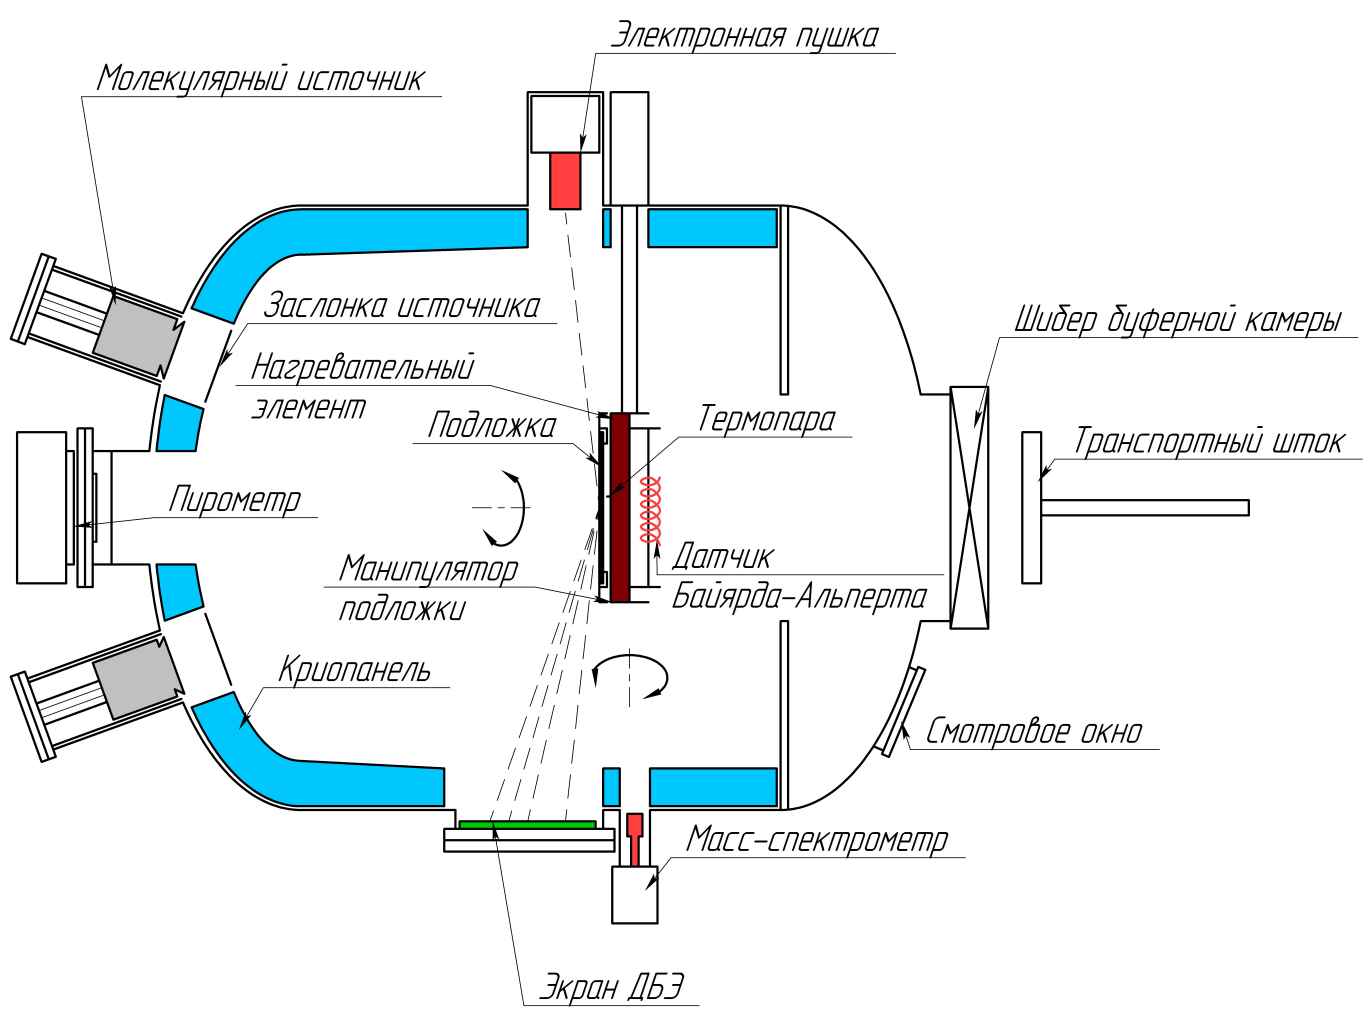
\includegraphics[width=1\linewidth]{Image_11}
} \caption{Схема ростовой камеры установки МПЭ Veeco GEN III, вид
сверху}\label{fig:Image_11} \end{figure}

Источник называют эффузионным, если длина свободного пробега молекул настолько
велика, что их взаимодействием в потоке можно пренебречь. Эффузионный источник
содержит тигель из пиролитического нитрида бора (pBN) с отверстием, в который
загружен испаряемый материал особой чистоты (\(\sim 99,99999\,\%\)). Тигель
окружен нагревательными элементами и охлаждающими трубками с потоком воды или
воздуха. Источники легирующих примесей Si и Be имеют только одну зону нагрева,
а источники элементов III группы имеют две зоны: основания тигля и апертурной
диафрагмы. Температура диафрагмы Ga и In источников поддерживается выше на
100~\si{\degreeCelsius} для предотвращения переконденсации материала на
диафрагму. Это необходимо для обеспечения стабильности потоков и снижения
плотности овальных дефектов. Температура диафрагмы Al источника поддерживается
ниже на 100~\si{\degreeCelsius} для предотвращения вытекания из тигля за счёт
смачивания поверхности pBN. Температура зон контролируется термопарами.
Величина потока регулируется нагревательными элементами и калибруется по
датчику потока перед каждым ростовым процессом. Источники оснащены
пневматическими заслонками для быстрого перекрытия потока.

Давление паров металлов III группы и легирующих примесей, в отличии от
элементов V группы, пренебрежимо мало при температуре синтеза~--- практически
все молекулы потока адсорбируются поверхностью. При росте планарных слоев поток
элементов V группы поддерживают в избытке для недопущения накопления
металлических капель на поверхности подложки из-за температурного разложения. В
таком случае скорость роста определяется потоком элементов III группы.

Управление потоками легколетучих P и As изменением температуры затруднено из-за
инерционности, поэтому крекерные источники P и As на выходе имеют игольчатый
клапан с 300 положениями между закрытым и полностью открытым. В отличие от
металлов III группы, которые испаряются в виде атомов, P и As испаряются в виде
многоатомных молекул \cite{Neave1980}. За игольчатым клапаном находится
крекерная трубка, нагреваемая до высоких температур. Тепловое инфракрасное
излучение поглощается молекулами, разрывая химические связи, таким образом
температура крекерной зоны определяет число атомов в молекулах потока.

В данной работе температура крекерного источника As составляла
600~\si{\degreeCelsius}, что соответствует потоку молекул As\textsubscript{4},
а температура крекерного источника P составляла 900~\si{\degreeCelsius}, что
соответствует потоку молекул P\textsubscript{2}. В конце крекерной зоны
находятся пневматические заслонки для быстрого перекрытия потока.

В крекерный источник P загружают менее химически активную красную аллотропную
модификацию. Давление пара белого P создаёт более стабильный поток, чем
давление пара красного P, поэтому внутри источника находится дополнительно
охлаждаемая область для переосаждения красного P в белый.

Молекулы N\textsubscript{2} имеют высокую энергию связи, поэтому для их
эффективного встраивания применяется источник, в котором поддерживается
высокочастотный (ВЧ) индуктивно-связанный плазменный разряд, в котором
молекулам сообщается дополнительная энергия. Метод роста с применением такого
источника называют молекулярно-пучковой эпитаксии с плазменной активацией азота
(ПА-МПЭ).

C обратной стороны манипулятора находится ионизационный вакуумный датчик
Байярда\,--\,Альперта, который может быть развернут в сторону источников. Он
предназначен для измерения эквивалентного давления пучка (ЭДП) попадающих на
подложку молекул. Из-за различной вероятности ионизации молекул корректно
сравнивать относительную величину потока только молекул одного типа. Различное
расположение источников относительно датчика потока также влияет на показание
датчика потока, на что указывает различная скорость роста при гомоэпитаксии
GaAs/GaAs(001) из разных источников Ga при одинаковых ЭДП в условиях избытка
As.

В некоторых случаях можно определить V/III соотношение ЭДП, при котором адатомы
находятся в стехиометрическом соотношении, наблюдая поверхностный фазовый
переход от обогащённой атомами III группы к обогащённой атомами V группы при
росте планарных слоев (например, в случае гомоэпитаксии GaP и GaAs).
Соотношение V/III ЭДП, при котором происходит поверхностный фазовый переход
зависит от температуры подложки, что, в свою очередь, объясняется зависимостью
отношения между величинами потоков десорбции адатомов V и III групп от
температуры. А следовательно соотношение V/III адатомов в общем случае
нелинейно зависит от соотношения ЭДП V/III.

Абсолютные значения и соотношения V/III ЭДП в схожих процессах на различных
установках МПЭ могут не совпадать, поэтому ориентация на значения потоков, при
которых адатомы находятся в стехиометрическом соотношении, может упростить
перенос ростовой технологии между установками.

\subsection{Дифракция быстрых электронов (ДБЭ)}\label{subsec:ch2/sec1/sub2}

Одно из преимуществ высокого вакуума~--- возможность использовать электронный
пучок для исследования структур в процессе роста. Сочетание относительной
простоты приборной системы и высокой поверхностной чувствительности сделало
метод дифракции быстрых электронов (ДБЭ) постоянным спутником метода МПЭ, а
систему ДБЭ~--- признаком, отличающим МПЭ от других эпитаксиальных методов.

Система ДБЭ состоит из электронной пушки, излучающей фокусируемый поток
электронов, и флуоресцентного экрана. Падая под скользящим углом, пучок
электронов с энергией \(\approx 15\)~\si{\kilo\electronvolt} рассеивается на
кристаллической решётке приповерхностных атомов в сторону флуоресцентного
экрана. По дифракционной картине можно судить о кристаллической структуре
поверхности, её реконструкции и структурном совершенстве, времени формирования
монослоя, морфологии наноструктур и наличии двойникования.

Рассеянные электроны конструктивно интерферируют при выполнении условий Лауэ:

\begin{equation} \label{eq:eq_2} \vec{k} - \vec{k_0} = m\vec{q}, \end{equation}
где \(\vec{k}\)~--- волновой вектор дифрагированной волны, \(\vec{k_0}\)~---
волновой вектор падающей волны, \(m\)~--- целое число, \(\vec{q}\)~--- вектор
обратной решётки.

В обратном пространстве через начало координат можно построить сферу отражения
радиусом \(| \vec{k} |\) с центром в начале вектора \(\vec{k}\). Данное
построение называют построением сферы Эвальда. Волновой вектор дифрагированных
волн, а с ним и картину дифракции, можно найти, построив вектора из центра
сферы Эвальда с концами в узлах обратной решётки, который пересекается сферой
Эвальда.

Обратная решётка от двумерной периодической структуры атомов представляет собой
множество бесконечно длинных стержней (тяжей), перпендикулярных к плоскости
атомов. Поэтому в случае кристаллической, атомарно гладкой поверхности сфера
Эвальда пересекает тяжи, что соответствует дифракционной картине из серии полос
с модулированной интенсивностью, наложенных на фон из-за неупругого рассеяния.

Если поверхность не гладкая, электроны рассеиваются сквозь неровности, в
результате чего образуется пятнистая дифракционная картина из рефлексов
(аналогично дифракции рентгеновских лучей на трёхмерной кристаллической
решётке), удлинённых в направлении нарушения кристаллической симметрии. Это
позволяет различить тонкие и широкие нанообъекты. Дифракция от аморфной
поверхности (например, от поверхностного оксида) формирует размытый диффузный
фон, а от поликристаллической поверхности~--- набор колец (аналогично
порошковым дифрактограммам).

Упорядочение поверхностных атомов может существенно отличаться от объёмного. В
результате поверхностной реконструкции формируется сверхструктура, базисная
ячейка которой обычно кратна элементарной ячейке исходной структуры. Когда углы
между векторами трансляции элементарных ячеек поверхности и подложки совпадают,
для обозначения сверхструктуры используют запись вида \begin{equation}
\label{eq:eq_3} \frac{a_{1s}}{a_{2b}} \times
\frac{a_{2s}}{a_{2b}}-R\phi\si{\degree}, \end{equation} где \(a_{1s}\) и
\(a_{2s}\)~--- вектора трансляции элементарной поверхностной ячейки, \(a_{1b}\)
и \(a_{2b}\)~--- вектора трансляции элементарной нижележащей ячейки,
\(\phi\si{\degree}\)~--- угол поворота ячейки.

Так как расстояние между дифракционными полосами обратно пропорционально
размеру элементарной ячейки поверхностной решётки, сверхструктура на картине
дифракции проявляется как набор полос между основными рефлексами.

Адсорбция на поверхности атомов также может способствовать поверхностному
фазовому переходу \cite{Bringans1993, Ji2007}. Адсорбируюсь, As пассивирует
поверхность Si\((111)7\)\(\times\)\(7\), образуя сверхструктуру
Si\((111)1\times1-\text{As}\) \cite{Patel1989, Bringans1992}, а P (из-за
больших поверхностных растягивающих напряжений) образует неупорядоченную
несоразмерную сверхструктуру
Si\((111)6\sqrt{3}\)\(\times\)\(6\sqrt{3}-R30\si{\degree}-\text{P}\)
\cite{Vitali1998, Siriwardena2017}. Ga образует различные сверхструктуры при
эквивалентной толщине менее монослоя, а при эквивалентных толщинах более
монослоя~--- образует капли (см.~рис.~\cref{fig:Image_12}) \cite{Park1988},
которые могут служить катализатором для роста в режиме ПЖК
(см.~подраздел~\cref{subsec:ch1/sec2/sub2}) или участвовать в капельной
эпитаксии (см.~подраздел~\cref{subsec:ch1/sec2/sub6}). Эквивалентный монослой
здесь означает \(6,8 \cdot 10^{14}\)~атомов\si{\per\centi\meter^{2}}~---
поверхностная плотность объёмного Si толщиной монослой на поверхности (111)
\cite{Kumar2010}.

\begin{figure}[ht] \centerfloat{
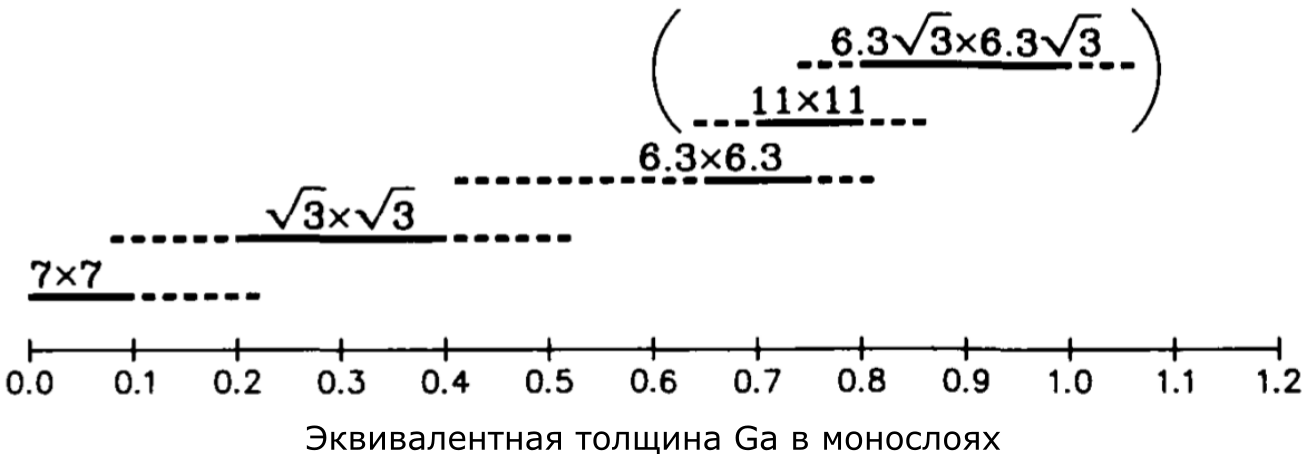
\includegraphics[width=0.8\linewidth]{Image_12} } \caption{Фазовая диаграмма Ga
на Si(111) \cite{Park1988}}\label{fig:Image_12} \end{figure}

В начале послойного роста, пока рост когерентен в области под электронным
пучком, интенсивность дифракционных линий осциллирует с периодом равным времени
формирования одного монослоя \cite{Harris1981}. Интенсивность рефлексов
максимальна, когда поверхность атомарно гладкая. Если зарождение происходит на
атомных террасах, то рассеяние от атомов поверхности и зародышей вызывает
деструктивную интерференцию, поэтому интенсивность рефлексов минимальна, когда
монослой заполнен наполовину. Осцилляции интенсивности не наблюдаются при росте
в режиме встраивания адатомов в край ступени «step-flow» (так как поверхность
сохраняет свою гладкость) и в случае роста объёмных наноструктур.

\section{Постростовые методы исследования}\label{sec:ch2/sec2}

\subsection{Растровая (РЭМ) и просвечивающая (ПЭМ) электронная
микроскопия}\label{subsec:ch2/sec2/sub1}

Иногда морфологию нанообъектов можно оценить методом оптической спектроскопии
даже если их размеры в одном или двух направлениях меньше дифракционного
предела, например, в целях определения длины, направления роста и плотности
ННК. Для получения изображений большего разрешения используются микроскопы с
пучком электронов вместо светового потока.

В растровых электронных микроскопах (РЭМ) сфокусированный электронный пучок
(диаметр \(\approx 1~\si{\nano\meter}\)) сканирует поверхность образца, при
взаимодействии с которым генерируются вторичные электроны и характеристическое
рентгеновское излучение, которые собираются детекторами. Интенсивность сигнала
зависит от природы вещества, что в некоторых случаях позволяет различать фазы с
разным химическим составом (например, включения GaPAs в ННК GaP), и топографии
в области взаимодействия. По спектру характеристического рентгеновского
излучения можно судить о концентрации химических элементов в образце.

В просвечивающих электронных микроскопах (ПЭМ) электронный поток, проходя
сквозь образец, неоднородно поглощается и рассеивается, после чего фокусируется
электронной оптикой на детекторе. Фокусное расстояние промежуточной линзы можно
менять так, чтобы на флуоресцентном экране фокусировалась или плоскость объекта
(для формирования его увеличенного изображения), или задняя фокальная плоскость
(для формирования картины микродифракции участка под электронным пучком).

Исследуемая область образца должна быть достаточно тонкой, порядка десятков нм,
поэтому образцы толще \(\approx 100~\si{\nano\meter}\) подготавливают
полировкой и ионным распылением.

Просвечивающий растровый электронный микроскоп (ПРЭМ)~--- вид ПЭМ, в котором
для увеличения разрешения пучок электронов фокусируют в точку размером
\(\approx 0,05~\si{\nano\meter}\), которой проводят растровое сканирование
поверхности образца.

При съёмке в светлопольном (bright field) режиме на детекторе собираются
электроны вблизи оси пучка. В этом случае на контраст в большей степени влияет
толщина, плотность, состав и кристаллическая структура исследуемого объекта:
области с большей толщиной и большим атомным номером имеют тёмный контраст
из-за неупругого рассеяния проходящих через образец электронов.

В темнопольном (dark field) режиме на детекторе, из-за введённой в фокальную
плоскость апертуры, собираются только определённые дифрагированные электроны. В
этом случае изображение чувствительно к кристаллической ориентации и дефектам
решётки.

Режим высокоразрешающей электронной микроскопии (ВРЭМ), в котором падающий
пучок электронов ориентирован параллельно оси зоны кристалла, позволяет изучать
кристаллическую структуру и дефекты с атомным разрешением
(\(\approx0,05~\si{\nano\meter}\)). Изображения ВРЭМ могут выглядеть, как
изображения атомной решётки, однако контраст создаётся интерференцией
дифрагированных лучей, поэтому изображения ВРЭМ следует интерпретировать с
осторожностью.

\subsection{Атомно-силовая микроскопия (АСМ)}\label{subsec:ch2/sec2/sub2}

Метод атомно-силовой микроскопии (АСМ) основан на регистрации взаимодействия
между поверхностью образца и остриём зонда для исследования рельефа и локальных
физических свойств поверхности. На воздухе данный метод позволяет исследовать
атомные ступени, а в условиях высокого вакуума в состоянии обеспечить реальное
атомное разрешение с визуализацией атомной реконструкции.

Зонд имеет конструкцию кантилевера, и представляет собой балку, один конец
которой жёстко закреплён, а на другом перпендикулярно выступает острие с
радиусом закругления 1--90~\si{\nano\meter}. Сила взаимодействия, действующая
на острие со стороны поверхности, изгибает балку, что регистрируется по
отклонению отражённого от балки луча лазера. Образец во время сканирования
перемещается пьезодвигателем во всех направлениях. В результате на изображении
АСМ каждой точке поверхности присваивается значение высоты рельефа.

Стремление улучшить латеральное разрешение привело к развитию полуконтактного
метода, при котором расстояние зонда до поверхности такое, что на него
действует как отталкивание, так и притяжение. Пьезоэлектрический вибратор, к
которому прикладывается гармоническое напряжение, возбуждает колебания
кантилевера на частоте близкой к резонансной с соответствующей амплитудой
свободных колебаний. Амплитуда колебаний зонда уменьшается с приближением до
поверхности из-за взаимодействия. Во время растрового сканирования из-за
неровностей рельефа расстояние зонда до поверхности изменяется, а
следовательно, и амплитуда колебаний. Это изменение расстояния компенсируется
системой обратной связи так, чтобы амплитуда колебания зонда оставалась
постоянной.

\subsection{Спектроскопия фотолюминесценции (ФЛ)}\label{subsec:ch2/sec2/sub3}

Метод спектроскопии фотолюминесценции (ФЛ) основан на явлении
фотолюминесценции~--- свечении, возбуждаемом светом. Это один из основных
методов изучения оптических свойств и структуры энергетических уровней
полупроводника.

Полупроводниковый образец облучается лазерным излучением с энергией фотонов
больше ширины запрещённой зоны, при этом генерируются неравновесные
электронно-дырочные пары, которые рассеивают часть своей энергии, а затем
рекомбинируют (как излучательно, так и безызлучательно). Длины волн и
интенсивность фотонов, испущенных данным образцом, регистрируются системой из
монохроматора и фотодетектора. Тепловые колебания кристаллической решётки
увеличивают вероятность безызлучательной рекомбинации, поэтому, как правило, ФЛ
при охлаждении образца становится ярче.

Электрон и дырка могут образовать экситон~--- связанное водородоподобное
состояние, устойчивое благодаря кулоновскому взаимодействию. Энергия
образования экситона меньше ширины запрещённой зоны на энергию связи электрона
и дырки, поэтому на спектрах ФЛ линии экситонного излучения смещены от края
зоны поглощения в сторону длинных волн. Свободный электрон может быть захвачен
нейтральным или ионизированным примесным атомом, образуя связанный на примеси
экситон. В таком случае линия экситонного излучения смещается в сторону длинных
волн от линии излучения свободных экситонов на энергию связи экситона с атомом
примеси.

В объёмных материалах экситонные состояния проявляются при низких температурах,
однако в наноразмерных структурах могут наблюдаться при комнатной температуре.

\subsection{Спектроскопия комбинационного рассеяния света
(КРС)}\label{subsec:ch2/sec2/sub4}

Комбинационное рассеяние света (КРС)~--- это неупругое рассеяние света
веществом с возбуждением или релаксацией собственных молекулярных колебаний
(мод). В случае твёрдого тела оно сопровождается рождением (стоксов процесс)
или уничтожением фононов (антистоксов процесс).

Как правило, в спектроскопии КРС проявляются колебания, при которых изменяется
поляризуемость связи, тогда как в инфракрасной спектроскопии проявляются
колебания с изменением дипольного момента связи. Величина рассеянной или
приобретённой фотоном энергии соответствует энергии фононов вблизи центра зоны
Бриллюэна. По интенсивности и величине сдвига можно сделать выводы о химическом
составе, кристаллической структуре и упругих напряжениях.

В резонансной спектроскопии КРС энергия возбуждающего фотона совпадает с
энергией электронного перехода материала образца. Электронное возбуждение может
повысить поляризуемость связи, и, следовательно, интенсивность сигнала КРС.

Установка спектроскопии КРС может быть объединена с установкой спектроскопии ФЛ
при условии высокой разрешающей способности монохроматора и детектора (\(<
1~\si{\per\centi\meter}\)).

\FloatBarrier
